\section{Preprocessing}
\label{sec:03_Preprocessing}
Ziel des Preprocessing ist es die Daten aufzubereiten das der
Informationsgehalt maximiert sowie Rauschen minimiert wird.
Desweiteren muessen die Daten so vorverarbeitet werden, dass diese
diese von den machine learning algorithmen ausgewertet werden können. 

Um das Untegrundrauschen zu minimieren koennten Bildausschnitten auf 
denen keine Wolken zu erkennen sind herausgeschnitten werden.
Stattdessen wird auf die Methode der Farb-Filter zurueckgegriffen, da dabei 
kein manuelle Nachbearbeitung der Fotos notwendig ist und somit ein höherer 
Automatisierungsgrad erreicht wird.

Dazu werden Bilder, die weniger als \SI{30}{\percent} der maximalen Helligkeit 
besitzen, verworfen. 
Anders als Beispielsweise bei einer Zeitschaltuhr laesst sich durch die
Seperation anhand des Helligkeitswert die Messzeit maximieren, da die 
Belichtung vom Monat als auch von der Wolkendecke abhaengig ist.
Fotos welche nicht dem Helligkeitscut entprechen werden noch bevor sie 
klassifiziert werden der Klasse 'schlechte Fotos' zugeordent um den 
Arbeitsaufwand geringer zu halten.

\begin{wrapfigure}{r}{0.5\textwidth}
		\centering
		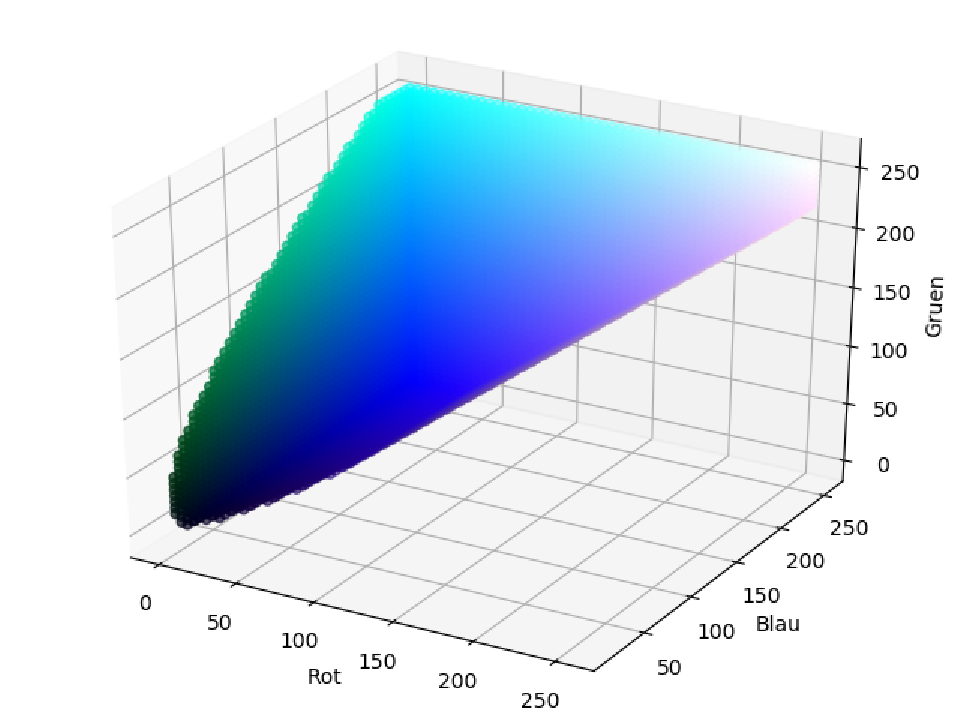
\includegraphics[width=0.49\textwidth]{pictures/cut_cube.pdf}
		\caption{Um den Winkel $\alpha$ zur Gruenebene geneigte Parabel im RGB 
				Farbraum, welche zu den Blauwerten geöffnet ist.}
				\label{fig:parabular}
\end{wrapfigure}
Das Wolkenspektrum hatt klar definierte Farben die Hauptsächlich aus Blau, Grau
und Weiß Tönen besteht.
Pixel die nicht zu diesem Spektrum gehörsn werden systematisch auf den
Minimalwert gesetzt.
Dazu wird der Farbraum in ein Rotiertes System $RGB'$ mittels der 
Rotationsmatrix $R_{\alpha}$ um den Nullpunkt gehdreht. 
Dem rotierten Farbraum $RGB'$ wird eine Parabel gelegt die Pixel verwirft, 
welche die Ungleichung 
\begin{equation}
		c' > (b' - x_0)^2 + x_1, \hspace{3em} c' \in (r', g')
\end{equation}
nicht erfüllen und anschließend die Parabel in den ungestrichenen Raum zurueck
rotiert.
Der Nullpunkt der Parabel wird mit den Helligkeitswerten verschoben.
Ein Beispiel ist fuer Alle  drei Kanäle in Abbildung \ref{fig:parabular} zu sehen.
Dadurch laesst sich ein grossteil der mitfotographierten Untergrunddaten durch
eine Konstanten Wert ersetzen \texttt{(0,0,0)}.
\begin{figure}
		\centering
		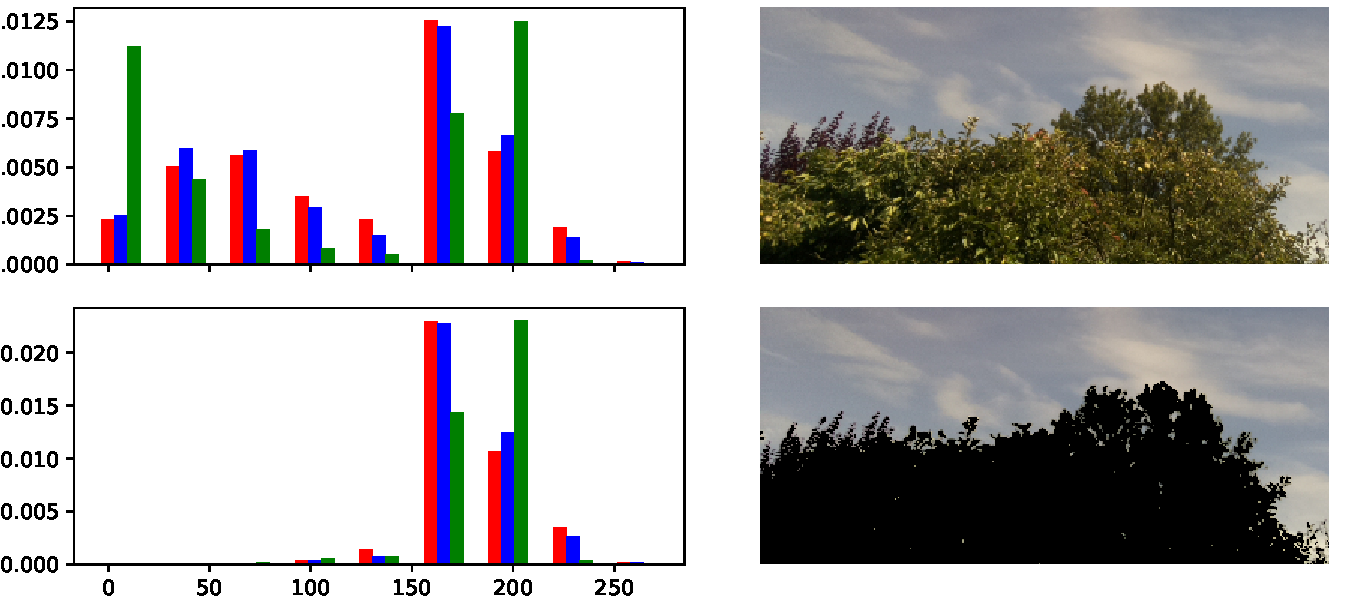
\includegraphics[width=0.95\textwidth]{pictures/cut_hist.pdf}
		\caption{Anhand des Farbspektrums geschwärzter Untergrund und die
		dazugehörigen Farbspektra zur Reduzierung des Umgebungsrauschens mit
		\texttt{bins = 10} zur Veranschauungszwecken.}
		\label{fig:name}
\end{figure}

Nachdem die Daten entsprechend aufbereitet wurden mussen sie noch in Form fuer
die Algorithmen gebracht werden. 
Dazu wird der Farbraum fuer den Random Forrest diskretisiert.
Durch mehrmaliges austesten kristallisierte sich eine Anzahl von 
\texttt{bins = 30} als die Diskretisierung mit den besten Ergebnissen heraus,
wobei die auf den Konstanten Wert gesetzten Untergrunddaten kein Teil des
Histogramms sind.
Fuer das Neuronale Netz werden die Bilddaten auf eins normiert und mittels 
eines \texttt{ImageDataGenerator} sequentiell aus den \texttt{JPG}-Dateien 
eingelesen. 
Dadurch laesst sich das Überlaufen des begrenzten Arbeitsspeicher auf Kosten 
der Trainingszeit, durch das wiederholte Laden der Daten von der Festplatte,
verhindern.


\section{Machine Learning}

Zur automatischen Bestimmung des Wolkentyps werden zwei verschiedene Algorithmen
verwendet. 
Einer von diesen ist der Random Forest weil dieser out of the box hinreichend schnell,
in der Auswertung und resourcendschonen ist.
Desweiteren wird ein CNN benutzt da dieses in der Laage ist auf den Wolkenformen
sowie dem Farbspektrum zu lernen. 

Beim training der Algorithmen stellte sich heraus das die Daten aufgrund des im
Kapitel \ref{sec:??} beschriebene Problem ein grossen Missmatch aufweisen. 
Daher aendert sich die Zielstellung bei der optimierung wesenltich.
Ziel ist vorerst nicht einen moeglichst hohe Genauigkeit zu erlangen um die
Wolkenklassifikation auf den PIs voran zu treiben sondern den Datensatz zu
erweitern und den Missmatch zu minimieren.
Dazu werden die Methoden genutzt um die Wolken welche nicht mit dem aktuellen
Label uebereinstimmen mittels dem Telegram Bot erneut zu ueberbruefen.
Desweiteren wird bei dem labeln neuer Daten immer ein Label vorgeschlagen
welches ubernommen oder per Hand gelabelt werden kann.
\begin{figure}
		\centering
		\includegraphics[width=\textwidth]{build/vorgehen.pdf}
		\caption{Modell fuer weiteres Vorgehen.}
		\label{fig:}
\end{figure}

Selbstverstaendlich bleibt das Optimierungskriterum die ACC wobei abgeleitete
Groessen wie der Loss oder confidence Werte kritisch bei Daten welche einen
Missmatch haben zu betrachten sind.

\subsection{Random Forest}%
\label{sub:random_forest}
\begin{wrapfigure}{r}{0.5\textwidth}
		\centering
		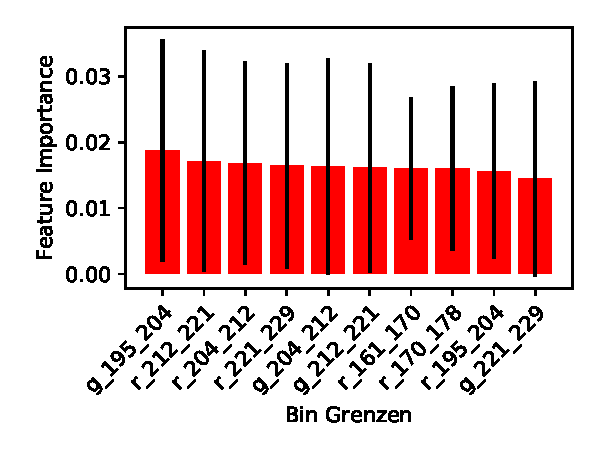
\includegraphics[width=0.5\textwidth]{./pictures/train_rf.pdf}
		\caption{}
		\label{fig:}
\end{wrapfigure}
Fuer das Training des Random Forrest koennen mehrere Parameter variiert werden.
Neben der Tiefe, der Anzahl an gezogenen Feature kann die Anzahl an
Entscheifungsbaeumen varriert werden.
Da die Methode des Random Forest jedoch durch einien hohe Anzahl an Baeumen
gegen Overfitting geschuetzt werden, werden die Tiefe der Baeume nicht weiter
beschraenkt und die Anzahl an gezogenen Featuren nicht weiter optimiert.
Desweiteren ist der histogrammierte Datensatz mit 30 bins pro Farbkanal fuer
machine learning algorithmen sehr niederdimensional.

\subsection{Convolution Neuronal Network}%
\label{sub:convolution_neuronal_network}

Die optimierung des Netzes steht unter der permisse die Architecture des Netzes
so einfach zu halten das die ACC maximal wird und die Parameteranzahl welche mit
der auswertungszeit correllieren kann gering bleibt. 
Beim Training mit der 'Cross Entropy' als Validation loss stellt sich wider
erwarten heraus das der validation loss bei guten Vorhersagen bei einem
Datensatz mit einem Missmatch steigt. 
Dies liegt daran wenn zum Beispiel bei dem waren label A der Datensatz das label
B hat. 
\begin{equation}
		H(p,q) = -\sum_x p(x) \log q(x)
\end{equation}
Somit wird die wahrscheinlichkeit $q(B)$ klein und die Kreuzentropie Gross.
Dies hat zur Folge das die Kreuzentropie bei Datensaetzen mit einem Missmatch
bei der Validierung fuer hohe ACC nicht abnimmt sondern groesse als zum Beispiel
beim Raten ist.
Das Uebertraining kann durch eine loss funktion welche nicht so sensible auf
Missmatches ist. 
Desweiteren wird im Rahmen der Moeglichkeiten der Missmatch der daten zu
minimieren.

\begin{figure}[h]
		\centering
		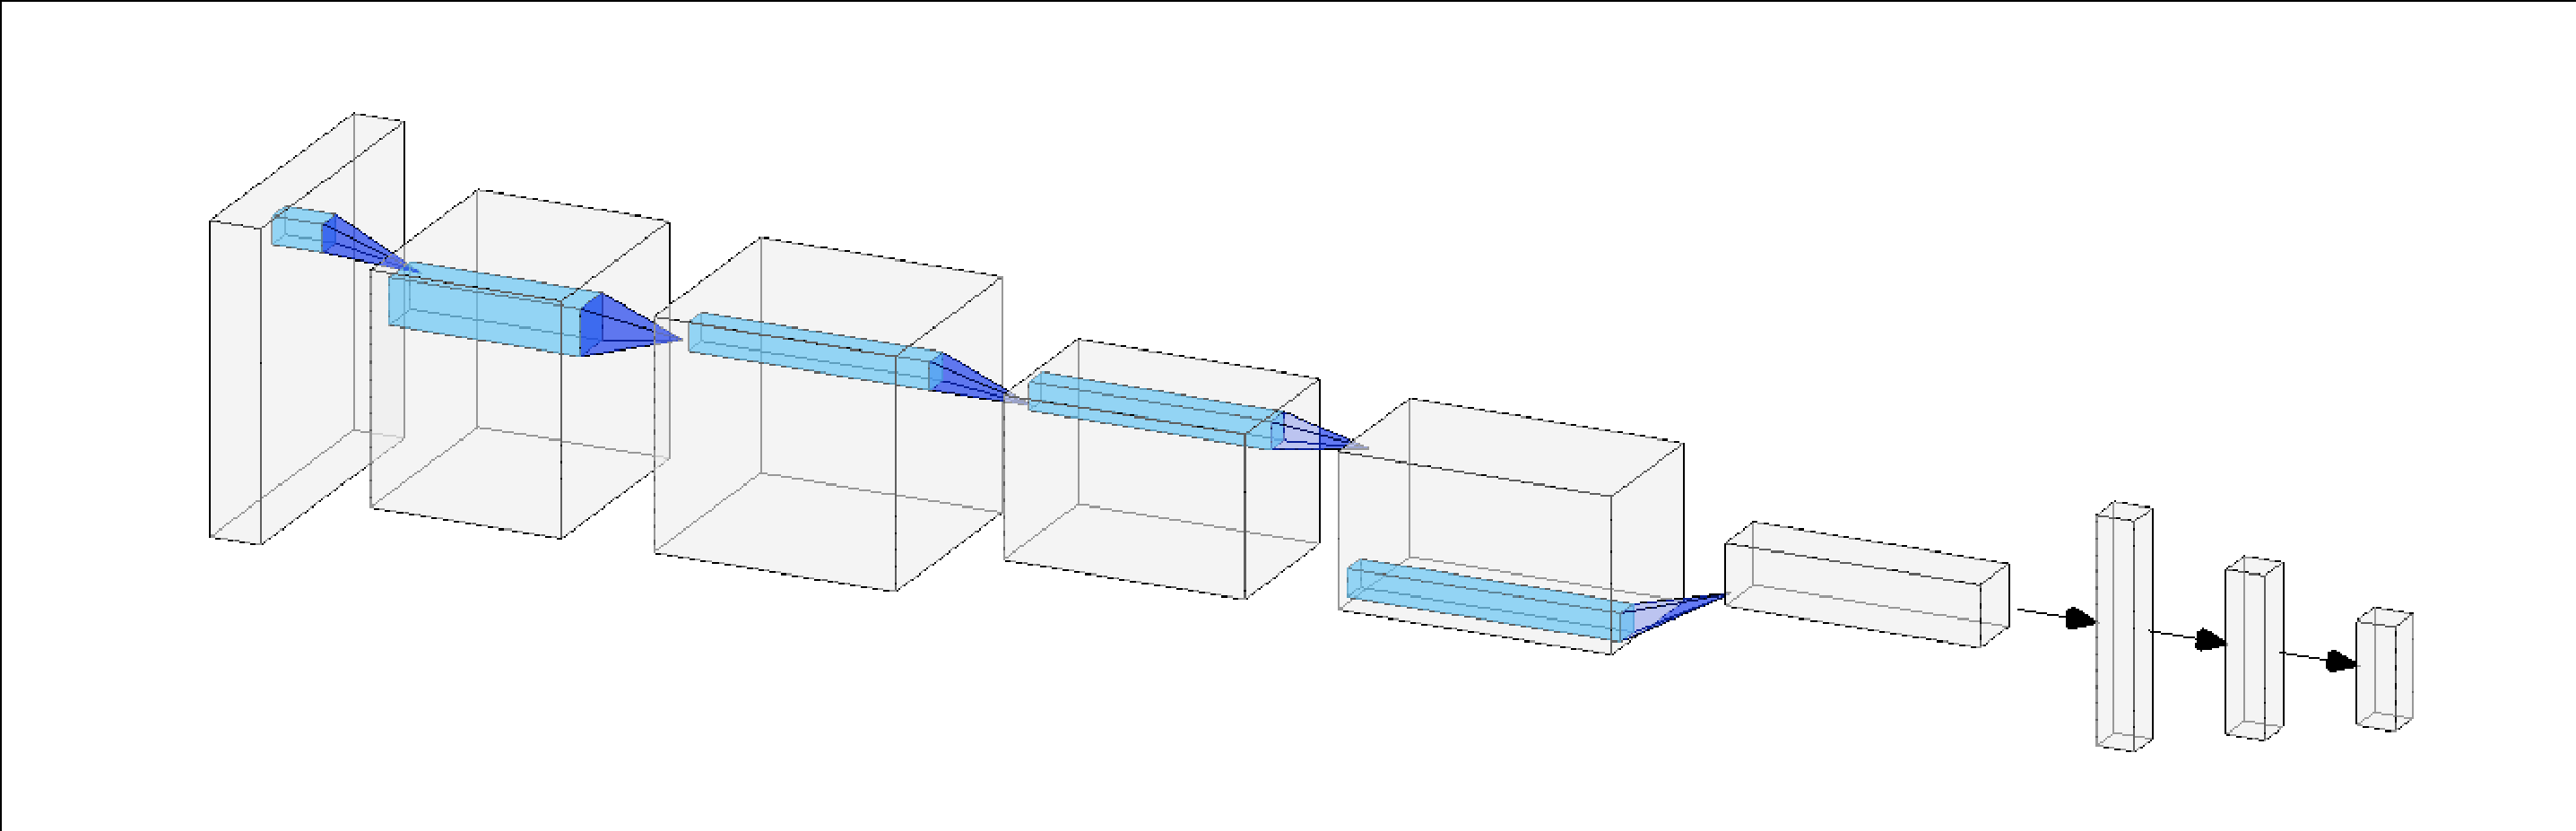
\includegraphics[width=0.8\textwidth]{pictures/architecture.pdf}
		\caption{}
		\label{fig:}
\end{figure}

Als architectur wird zunächst eine AveragePooling schicht gewählt um die
Dimesonalität des Bildes zu verringern.
Anschließend folgen drei Convolution Schichten die der Faltung des Bildes
dienen. 
Zwischen den Convolution schichten werden die Dimesonalität durch jeweils einer
MaxPooling Schicht verringert. 
Anschließend folgen zwei Dense Schichten die der Verarbeitung der
hochdimensionalen Daten dient. 
Diese werden durch jeweils einer Dropout und Noise Schicht regularisiert. 
Abschließend folgt eine Dense schicht mit der Anzahl an neuronen der
Zielklassen.
Fuer die Kernel sowie die Dens schichten wird die Relu funktion als
Aktivierungsfunktion genutzt.
Fuer die letzte Schicht wird entsprechend die Sigmoid funktion verwendet um die
Vorraussagen glatt zu machen und auf 1 zu normieren.
